\question[10] A partir de la gráfica de la figura \ref{fig:SINMAT1_U3_AC75_IMG2} que muestra el registro de la distancia que recorre un corredor con respecto al tiempo en uno de sus entrenamientos, escribe la cantidad correcta en el cuadro de texto.
\begin{figure}[H]
    \centering
    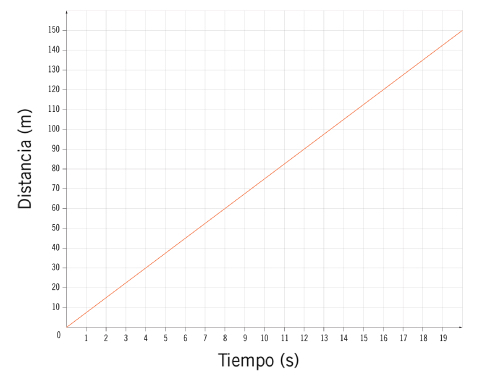
\includegraphics[width=0.75\textwidth]{../images/SINMAT1_U3_AC75_IMG2.jpg}
    \caption{Tabla de precios de los direrentes reciclables.}
    \label{fig:SINMAT1_U3_AC75_IMG2}
\end{figure}
\begin{parts}
    \subfile{../parts/question075b01}
    \subfile{../parts/question075b02}
    \subfile{../parts/question075b03}
    \subfile{../parts/question075b04}
    \subfile{../parts/question075b05}

\end{parts}